\subsection{BIDUAL}

Let E be a left A-module. The dual E** of the dual E* of E is called the bidual of E; it is also a left A-module (no. 3). For all \(x \in \mathbf{E}\) , it follows from no. 3, formulae (10) and (12), that the mapping \(x^* \mapsto \langle x, x^* \rangle\) is a linear form on the right A-module E*, in other words an element of the bidual E**, which we shall denote by \(\tilde{x}\) ; moreover, it follows immediately from (9) and (11) (no. 3) that the mapping \(c_{\mathbf{E}}: x \mapsto \tilde{x}\) of E into E** is linear; this mapping will be called canonical; in general, it is neither injective nor surjective, even when E is finitely generated (cf.~Exercise 9(e) and § 7, no. 5, Theorem 6).

An A-module E is called reflexive if the canonical homomorphism \(c_{E}:E \rightarrow E^{**}\) is bijective.

Let F be a second left A-module; for every linear mapping \(u: E \to F\) , the mapping \(t(tu): E^{**} \to F^{**}\) , which will also be denoted by \({}^{tt}u\) , is linear and the diagram

\begin{enumerate}
\def\labelenumi{(\arabic{enumi})}
\setcounter{enumi}{26}
\tightlist
\item
\end{enumerate}

\pandocbounded{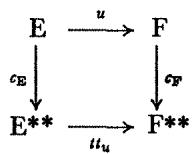
\includegraphics[keepaspectratio]{images/part002_cca49df6.jpg}}

is commutative, as follows immediately from the definitions and formula (15) giving the transpose of a linear mapping.

PROPOSITION 13. If E is a free module (resp. a free module with a finite basis), the canonical mapping \(c_{E}:E \rightarrow E^{**}\) is injective (resp. bijective).

Let \((e_t)_{t \in \mathbb{T}}\) be a basis of \(\mathbf{E}\) and let \((e_t^*)\) be the family of corresponding coordinate forms; by definition, if \(x \in \mathbf{E}\) is such that \(\tilde{x} = 0\) , then \(\langle x, e_t^* \rangle = 0\) for all \(t \in \mathbb{T}\) , in other words all the coordinates of \(x\) are zero, hence \(x = 0\) . Suppose further that \(\mathbf{T}\) is finite; since \(\langle \tilde{e}_t, e_{t'}^* \rangle = \delta_{tt'}\) , \((\tilde{e}_t)\) is the dual basis of \((e_t^*)\) in \(\mathbf{E}^{**}\) and, as \(c_{\mathbf{E}}\) transforms a basis of \(\mathbf{E}\) into a basis of \(\mathbf{E}^{**}\) , \(c_{\mathbf{E}}\) is bijective (§ 1, no. 11, Corollary 3 to Proposition 17). We have moreover proved:

COROLLARY 1. Let E be a free A-module with a finite basis; for every basis \((e_t)\) of E, \((c_{\mathbf{E}}(e_t))\) is the dual basis of the basis \((e_t^*)\) of E* dual to \((e_t)\) .

In this case it is said that \((e_t)\) and \((e_t^*)\) are two dual bases of one another.

COROLLARY 2. If E is a free A-module with a finite basis, every finite basis of \(\mathbf{E}^*\) is the dual basis of a basis of \(\mathbf{E}\) .

It suffices to consider in E** the dual basis of the given basis and canonically to identify E with E**.

COROLLARY 3. Let E, F be two A-modules each with a finite basis, E (resp. F) being canonically identified with its bidual E** (resp. F**). Then, for every linear mapping \(u: \mathbf{E} \to \mathbf{F}\) , \(^{tt}u = u\) .

This follows immediately from the commutativity of diagram (27).

COROLLARY 4. If P is a projective module (resp. a finitely generated projective module) the canonical mapping \(c_{\mathbf{P}}: \mathbf{P} \to \mathbf{P}^{**}\) is injective (resp. bijective).

We shall use the following lemma:

Lemma 1. Let M, N be two supplementary submodules in an A-module E and i: M → E, j: N → E the canonical injections. Then the diagram

\begin{enumerate}
\def\labelenumi{(\arabic{enumi})}
\setcounter{enumi}{27}
\tightlist
\item
\end{enumerate}

\pandocbounded{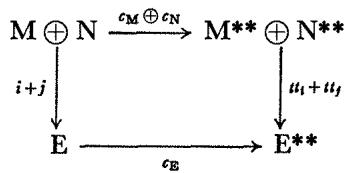
\includegraphics[keepaspectratio]{images/part002_690a791a.jpg}}

is commutative.

By definition, for \(x \in \mathbf{M}\) , \(y \in \mathbf{N}\) , \(z^{*} \in \mathbf{E}^{*}\) ,

\[
\begin{array}{r l} \langle c _ {\mathrm{E}} (i (x) + j (y)), z ^ {*} \rangle & = \langle i (x) + j (y), z ^ {*} \rangle \\ & = \langle i (x), z ^ {*} \rangle + \langle j (y), z ^ {*} \rangle \\ & = \langle x, ^ {t} i (z ^ {*}) \rangle + \langle y, ^ {t} j (z ^ {*}) \rangle \\ & = \langle c _ {\mathrm{M}} (x), ^ {t} i (z ^ {*}) \rangle + \langle c _ {\mathrm{N}} (y), ^ {t} j (z ^ {*}) \rangle \\ & = \langle^ {t t} i (c _ {\mathrm{M}} (x)) + ^ {t t} j (c _ {\mathrm{N}} (y)), z ^ {*} \rangle . \end{array}
\]

This being so, if E is a free module (resp. a free module with a finite basis), \(c_{E}\) is injective (resp. bijective); on the other hand, it follows from no. 6, Proposition 10, that \(^{tt}i \oplus ^{tt}j\) is bijective; the commutativity of diagram (28) then implies that \(c_{M} \oplus c_{N}\) is injective (resp. bijective) and so therefore are \(c_{M}\) and \(c_{N}\) (§ 1, no. 6, Corollary 1 to Proposition 7), whence the corollary, taking account of no. 2, Proposition 4.

